\section{Einführung}

\begin{frame}{Was ist \LaTeX?}
  \begin{itemize}
    \item \emph{Programmiersprache} zum Setzen von Text
    \item Kein WYSIWYG, es werden Befehle und Inhalt in normale Text-Dateien geschrieben.
    \item Kompiler überträgt \LaTeX-Code in ein Ausgabedokument (meist PDF)
    \item open-source mit zahlreichen Erweiterungsmöglichkeit (Pakete)
  \end{itemize}
\end{frame}

\begin{frame}{Warum \LaTeX?}
  \begin{itemize}
    \item hervorragender Text- und Formelsatz
    \item automatisierte Erstellung von Inhalts- und Literaturverzeichnis
    \item \TeX-Dateien sind reine Text-Dateien \\
          $\Rightarrow$ gut für Versionskontrolle geeignet
    \item sehr gute Vorlagen für wissenschaftliches Arbeiten
    \item aber auch: Briefe, Notensatz, Präsentationen (auch diese)
    \item ausgezeichnete Dokumention
    \item erweiterbar durch zahlreiche und mächtige Pakete
    \item auf allen geläufigen Betriebssystemen verfügbar
    \item Ausgabe direkt als PDF mit Hyperlinks
  \end{itemize}
\end{frame}

\begin{frame}{Geschichte}
  \begin{columns}
    \begin{column}{0.75\textwidth}
      \begin{itemize}
        \item \TeX
          \begin{itemize}
            \addtolength{\itemsep}{0.5\baselineskip}
            \item Geschrieben von Donald E. Knuth 1978, um sein Buch \enquote{The Art of Computer Programming} zu setzen
            \item auf Aussprache achten!
            \item Version (2014) $3.14159265 → \mathup{π}$
            \item viele Erweiterungen: \eTeX, pdf\TeX, \XeTeX, \LuaTeX
          \end{itemize}
        \item \LaTeX
          \begin{itemize}
            \addtolength{\itemsep}{0.5\baselineskip}
            \item Geschrieben von Leslie Lamport 1984
            \item Version (1994) \LaTeXe
            \item \LaTeX3 seit Anfang der Neunziger in Arbeit…
          \end{itemize}
      \end{itemize}
    \end{column}
    \begin{column}{0.25\textwidth}
      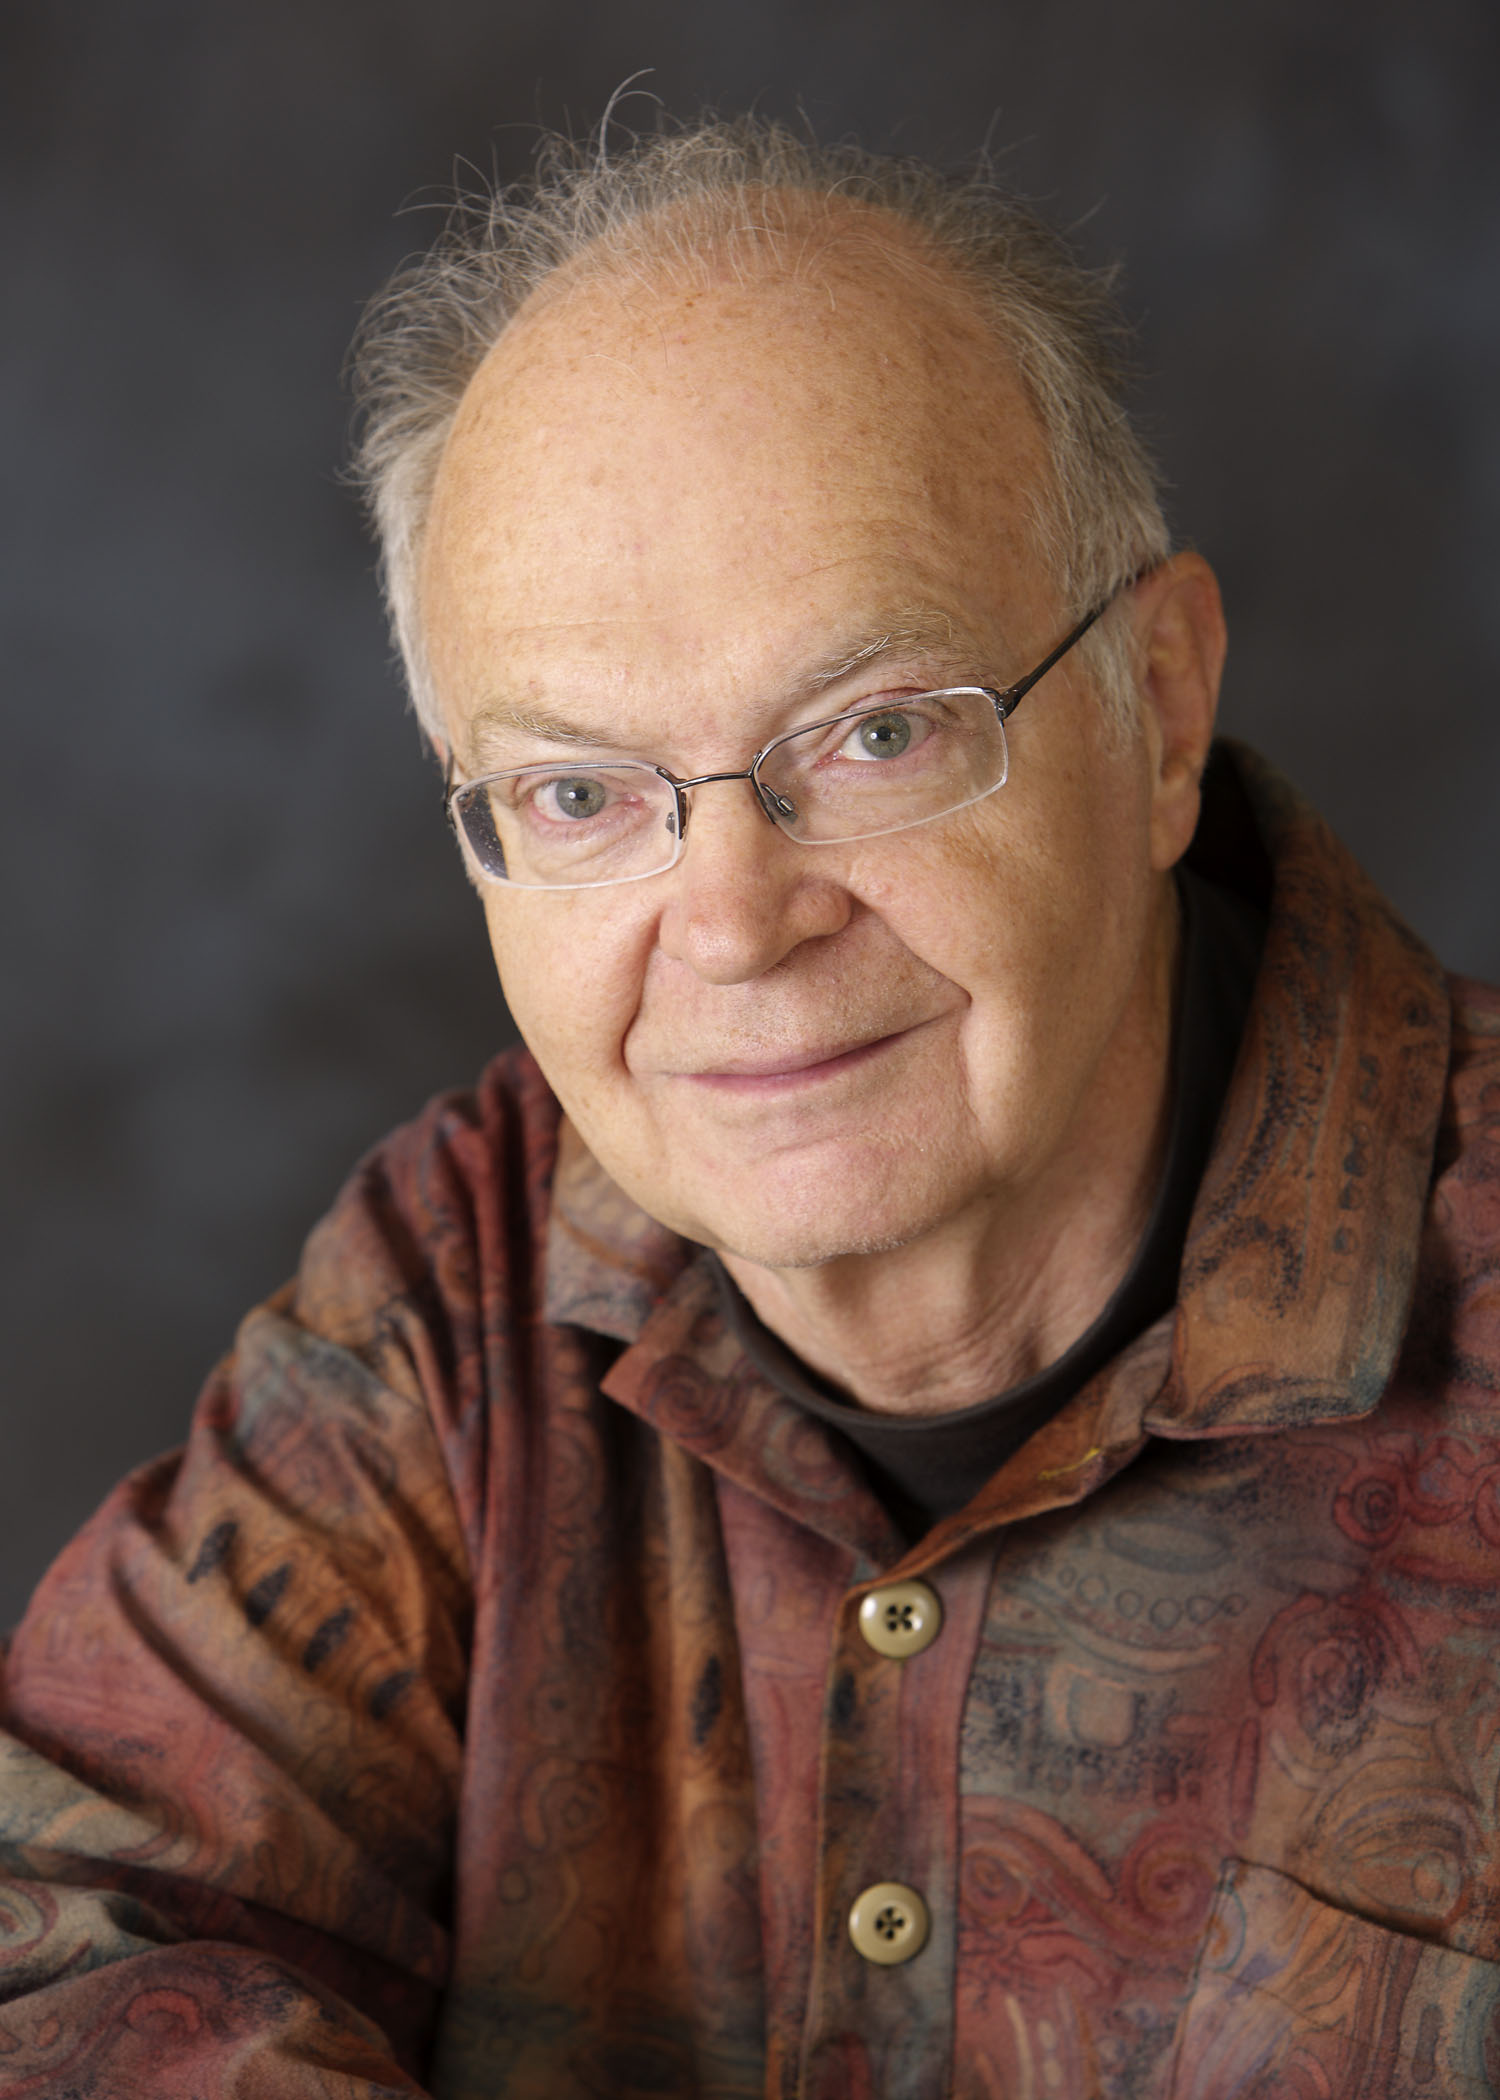
\includegraphics[height=0.45\textheight]{figures/knuth.jpg}\\
      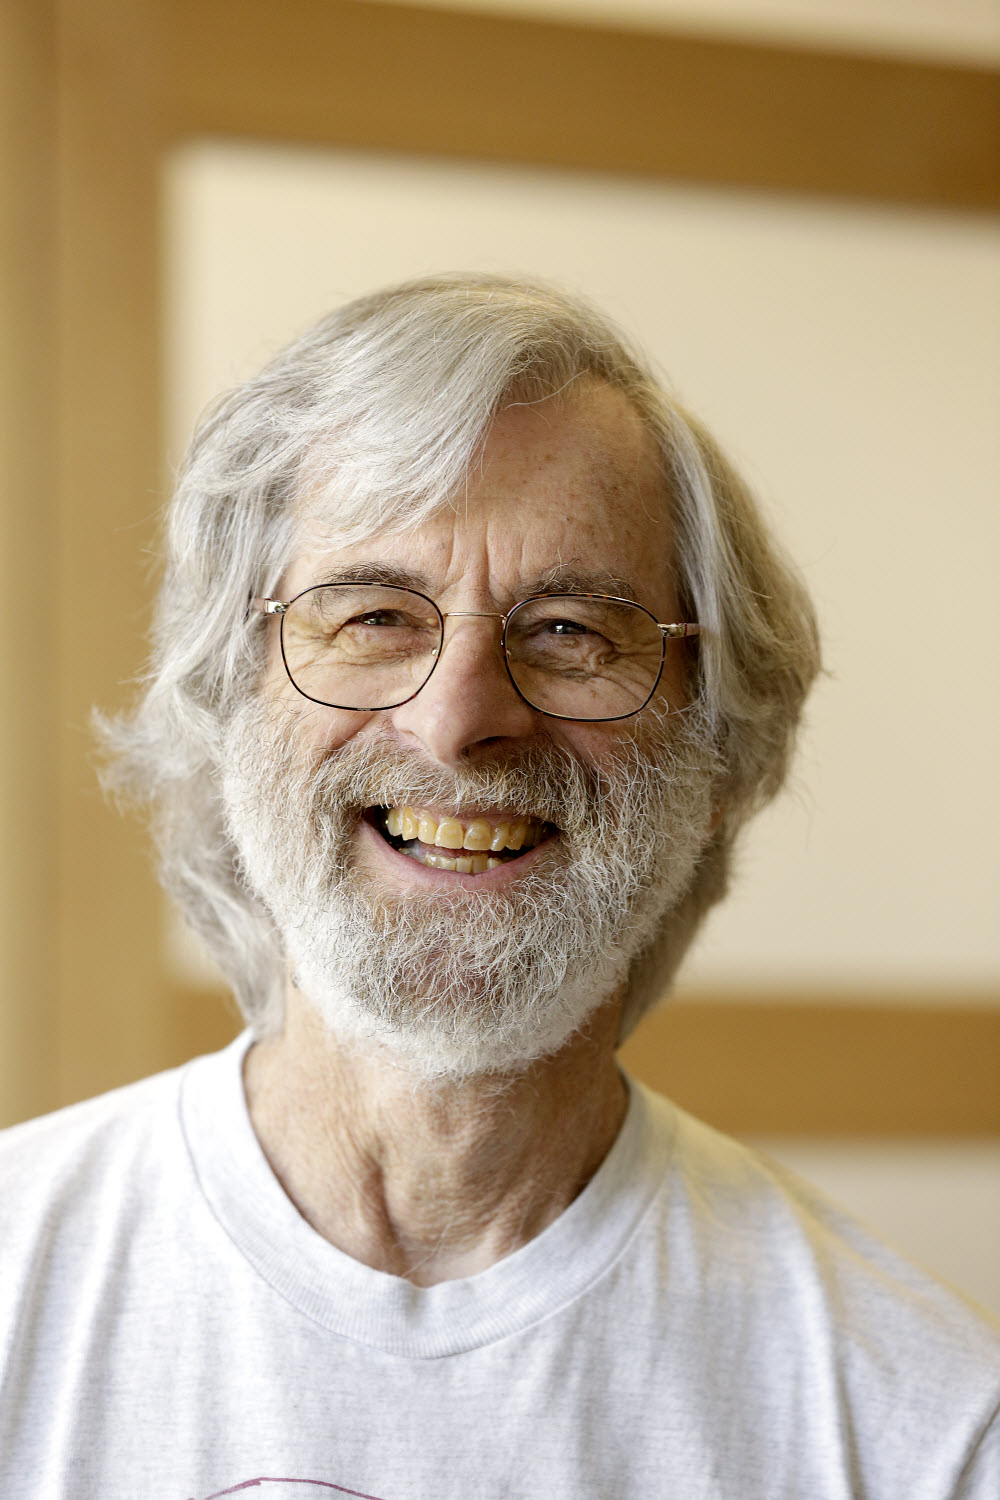
\includegraphics[height=0.45\textheight]{figures/lamport.jpg}
    \end{column}
  \end{columns}
\end{frame}

\begin{frame}
  \centering
  \only<1>{
    \includegraphics[height=0.95\textheight]{figures/engines-few.pdf}
    \hspace{1.15em}
  }
  \only<2,3>{
    \includegraphics[height=0.95\textheight]{figures/engines-many.pdf}
  }
  \begin{tikzpicture}[remember picture,overlay]
    \tikzset{shift={(current page.center)}}
    \node at (-4.3,1.3) {
      \TeX-Engines
    };
    \only<3>{
      \node (here) at (-4.3,-2.8) {
        Sie sind hier
      };
      \draw [->, >=Stealth] (here.east) -- ++(1.65,-0.75);
    }
  \end{tikzpicture}
\end{frame}

\begin{frame}[t]
  \centering
  \only<1>{
    \includegraphics[height=5.45em]{figures/formats-few.pdf}
    \hspace{0.5em}
  }
  \only<2,3>{
    \includegraphics[height=0.95\textheight]{figures/formats-many.pdf}
  }
  \begin{tikzpicture}[remember picture,overlay]
    \tikzset{shift={(current page.center)}}
    \node at (-4.3,2.3) {
      \TeX-Formate
    };
    \only<3>{
      \node (here) at (-4.3,-0.8) {
        Sie sind hier
      };
      \draw [->, >=Stealth] (here.east) -- ++(3.05,0);
    }
  \end{tikzpicture}
\end{frame}
